\documentclass{article}
\usepackage{tikz}
\usepackage{siunitx}
\usepackage{forest}
\usepackage{cleveref}
\usetikzlibrary{arrows.meta,shapes,positioning}
\usepackage{../themeKonstanz}
\usepackage{pgfplots}

\usetikzlibrary{arrows,shapes,positioning}
\usetikzlibrary{decorations.markings}

\tikzset{fontscale/.style = {font=\relsize{#1}}
    }
\usetikzlibrary{arrows.meta,shapes,positioning}
\tikzset{MyArrow/.style={single arrow, draw, minimum width=8mm, minimum height=5mm,
                         inner sep=0mm, single arrow head extend=1mm}}

\begin{document}
\begin{figure}
    \centering
    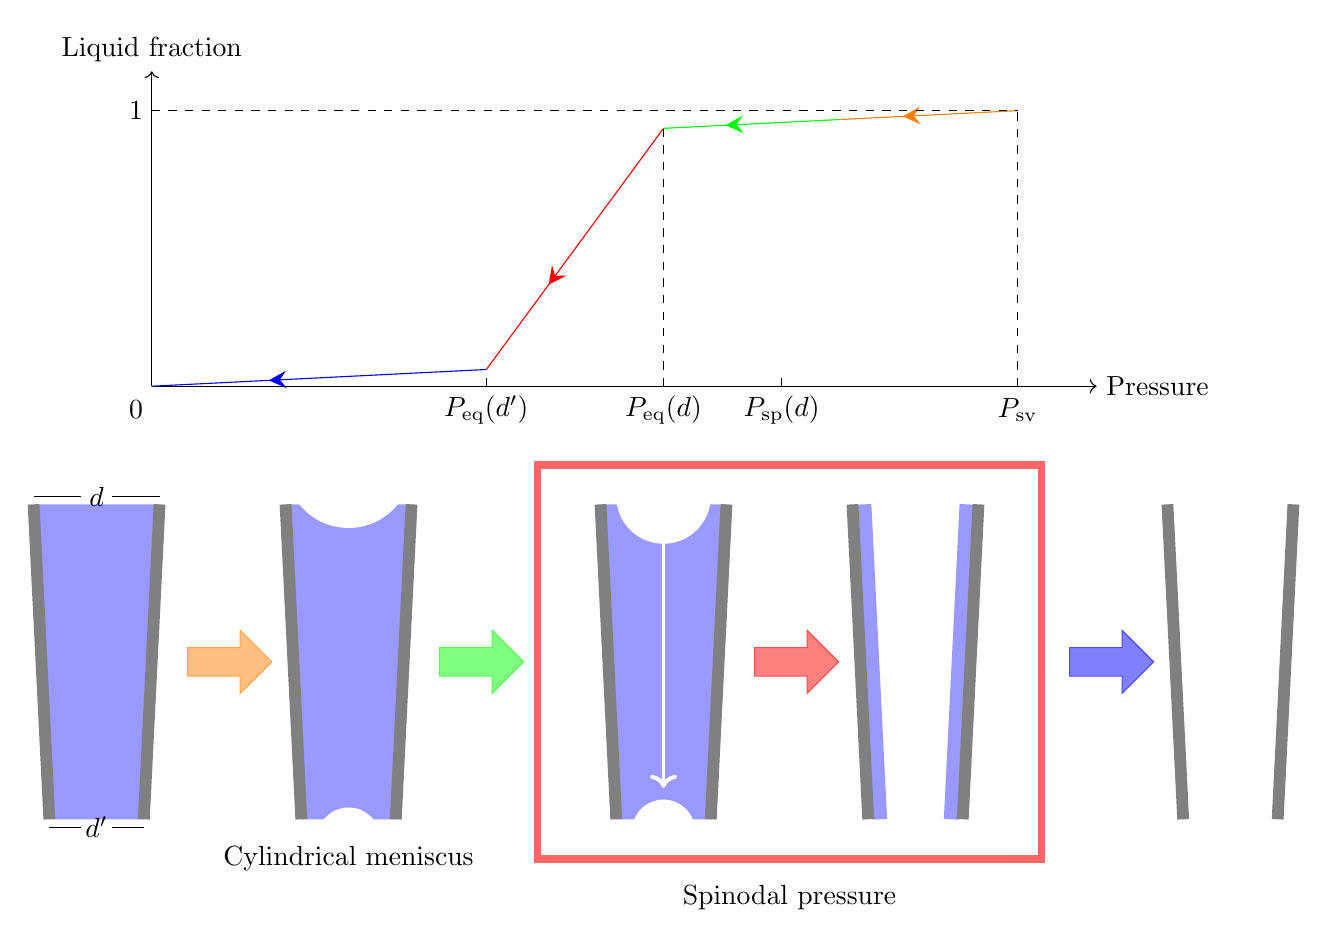
\begin{tikzpicture}[pore/.style = {line width = 0.15cm, color = gray},
                        film/.style = {line width = 0.18cm, color = blue!40},
                        thick_film/.style = {line width = 0.3cm, color = blue!40},
                        graph_label/.style={color = gray, line width = 0.05cm},
                        pore_collapse/.style = {color = blue!50, line width = 0.07cm, ->},
                        MyArrow/.style={single arrow, draw, minimum width=8mm, minimum height=5mm,
                        inner sep=0mm, single arrow head extend=1mm}]
        \pgfdeclarelayer{bg}    % declare background layer
        \pgfdeclarelayer{bbg}    % declare backbackground layer
        \pgfsetlayers{bbg,bg,main}  % set the order of the layers (main is the standard layer)
        \tikzstyle arrowstyle=[scale=2]
        \tikzstyle directed=[postaction={decorate,decoration={markings,
            mark=at position .65 with {\arrow[arrowstyle]{stealth}}}}]
        \begin{scope}
            \foreach \Xcoor in {0, 3.2, 7.2, 10.4, 14.4}
            \draw[pore] (\Xcoor + 0.2,0) -- (\Xcoor,4);
            \foreach \Xcoor in {1.6, 4.8, 8.8, 12, 16}
            \draw[pore] (\Xcoor - 0.2,0) -- (\Xcoor,4);
            \draw (0.6,4.1) -- (0,4.1); 
            \draw (1,4.1) -- (1.6,4.1); 
            \node at (0.8,4.1) {$d$};
            \draw (0.6,-0.1) -- (0.2,-0.1); 
            \draw (1,-0.1) -- (1.4,-0.1); 
            \node at (0.8,-0.1) {$d'$};
            \node[draw = orange!70, fill = orange!50, MyArrow] at (2.4, 2) {\phantom{arrow}};
            \node[draw = green!70, fill = green!50, MyArrow] at (5.6, 2) {\phantom{arrow}};
            \node[draw = red!70, fill = red!50, MyArrow] at (9.6, 2) {\phantom{arrow}};
            \node[draw = blue!70, fill = blue!50, MyArrow] at (13.6, 2) {\phantom{arrow}};
            %
            \draw[color = red!60, line width = 0.1cm] (6.4,-0.5) -- (12.8,-0.5) -- (12.8,4.5) -- (6.4,4.5) -- cycle;
            \node at (9.6,-1) {Spinodal pressure};
            \node at (4,-0.5) {Cylindrical meniscus};
            \begin{pgfonlayer}{bg}    % select the background layer
                %full pore
                \fill[blue!40] (0.2,0) -- (0,4)  -- (1.6,4) -- (1.4,0) -- cycle ;
                %full pore with menisci
                \fill[blue!40] (3.4,0) -- (3.2,4)  -- (4.8,4) -- (4.6,0) -- cycle ;
                \path [draw = none, fill = white](3.2,4.5) arc[start angle = -180, end angle = 0, radius=0.8];
                \path [draw = none, fill = white](3.6,-0.25) arc[start angle = 180, end angle = 0, radius=0.4];
                %emptying pore
                \fill[blue!40] (7.4,0) -- (7.2,4)  -- (8.8,4) -- (8.6,0) -- cycle ;
                \path [draw = none, fill = white](7.4,4.1) arc[start angle = -180, end angle = 0, radius=0.6];
                \path [draw = none, fill = white](7.6,-0.15) arc[start angle = 180, end angle = 0, radius=0.4];
                \draw[color = white, ->, line width = 0.5mm] (8,4) -- (8,0.4) ;
                %filmed pore
                \draw[film] (10.75,0) -- (10.55,4);
                \draw[film] (11.65,0) -- (11.85,4);
            \end{pgfonlayer}
        \end{scope}
        \begin{scope}[xshift = 1.5cm, yshift=5.5cm]
            \draw[->] (0,0) -- (0,4) node[anchor=south] {Liquid fraction};
            \draw[->] (0,0) -- (12,0) node[anchor=west] {Pressure};
            %orange
            \draw[color = blue, directed] (4.25,0.2125) -- (0,0);
            %red
            \draw[color = red, directed] (6.5,3.275) -- (4.25,0.2125);
            %green
            \draw[color = green, directed] (8.75,3.3875) -- (6.5,3.275);
            %blue
            \draw[color = orange, directed] (11,3.5) -- (8.75,3.3875);
            %DASHED
            \draw[dashed] (0,3.5) -- (11,3.5);  %1
            \draw[dashed] (11,0) -- (11,3.5);  %psat
            \draw[dashed] (6.5,0) -- (6.5,3.275);  %psp
            \draw[dashed] (8,0) -- (8,0.15);  %peq
            \draw[dashed] (4.25,0) -- (4.25,0.15);  %peq
            %labels
            \node at (-0.2,-0.3) {$0$};
            \node at (-0.2,3.5) {$1$};
            \node at (11,-0.3) {$P_\mathrm{sv}$};
            \node at (4.25,-0.3) {$P_\mathrm{eq}(d')$};
            \node at (6.5,-0.3) {$P_\mathrm{eq}(d)$};
            \node at (8,-0.3) {$P_\mathrm{sp}(d)$};
        \end{scope}
    \end{tikzpicture}
    \caption{Desorption isotherm of a funnelled cylindrical pore. Below, the processes inside the pore are illustrated. The colors of the broad arrow's colors correspond to the pressure ranges of the isotherm in the same color. Significant is the desorption at equilibrium pressure which yields a slope depending on the funnelization angle.}
    \label{fig:perf-cyl-pores-cond}
\end{figure}
\end{document}

%Evaporation process inside a funnelled cylindrical pore. Decreasing vapor pressure around a filled pore, negative spherical menisci form on both ends. Upon reaching equilibrium pressure of the larger pore radius $r$, the pore starts to empty from the large end. both sides only leaving a film on the inside. The film evaporates continuously approaching saturated vapor pressure at which it disappears completely. The graph shows the liquid fraction inside the pore depending on the current vapor pressure. The slopes before and after the evaporation at equilibrium pressure imply the appearance of the menisci an the evaporation of the film.